\documentclass{article}

\usepackage{graphicx}
\usepackage{hyperref}
\usepackage{tikz}
\tikzset{
  treenode/.style = {shape=rectangle, rounded corners,
                     draw, align=center,
                     top color=white, bottom color=gray!20},
  root/.style     = {treenode, bottom color=blue!30},
  env/.style      = {treenode, font=\ttfamily\normalsize},
  dummy/.style    = {circle,draw}
}
\begin{document}
\setlength{\parskip}{1em}
\setlength{\parindent}{0em}

\title{Project: REST-Server for Alfafold instance}
\section{Overview}
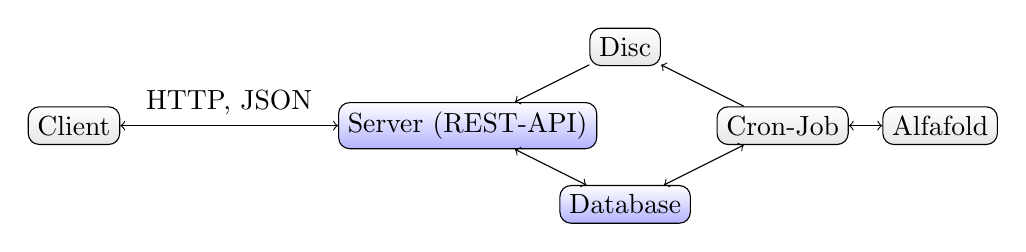
\begin{tikzpicture}
%Nodes
\node[treenode]  (Client) at (0,1) {Client};
\node[root]  (Server) at (5,1) {Server (REST-API)};

\node[root]  (Database) at (7,0) {Database};
\node[treenode]  (Disc) at (7,2) {Disc};

\node[treenode]  (Sheduler) at (9,1) {Cron-Job};
\node[treenode]  (Alfafold) at (11,1) {Alfafold};

%Lines
\draw[<->] (Client) edge node[thick, auto] {HTTP, JSON} (Server);

\draw[<-] (Server) edge node[thick, auto] {} (Disc);
\draw[<->] (Server) edge node[thick, auto] {} (Database);

\draw[<-] (Disc) edge node[thick, auto] {} (Sheduler);
\draw[<->] (Database) edge node[thick, auto] {} (Sheduler);

\draw[<->] (Sheduler) edge node[thick, auto] {} (Alfafold);
\end{tikzpicture}

\subsection{Description}
You will implement a REST-API server using the library Flask (or similar library) with Python.
The server will present the data to the client and receive data from the client encoded in JSON.
The data will be stored in a MySQL-database. A description of some tables you will find in section \ref{ch!database}. You will extend the database as needed.

On the server is a cron-job running which will check the database and give
Alfafold the next task according to the given settings. When Alfofold is
finished with the work, the cron-job will save the resulting \texttt{.zip}
file in the file-system. The cron-job will update the entry for the current
task in the database according to the current state (waiting $\to$ working $\to$ finished) give a path to the log-file and the path to the results-file.

In the first steps you will concentrate on the tasks.
When it is proved that your server can control the tasks you will work on user control.


\subsection{Workpackages}
\begin{minipage}{0.45\textwidth}
Step 1: Task
  \begin{itemize}
  \item create
  \item list
  \item edit
  \item delete
  \item activate
  \item deactivate
  \item download results
  \end{itemize}
\end{minipage}
\hfill
\begin{minipage}{0.45\textwidth}
Step 2: User
  \begin{itemize}
  \item create
  \item list
  \item edit
  \item delete
  \item login
  \item logout
  \item change password
  \end{itemize}
\end{minipage}

\subsection{Database Tables}\label{ch!database}
\subsubsection{Table 'af\_tasks'}
Entries for this table will be created by the frontend.

fields:
\begin{itemize}
\item \texttt{id} (Int, Key) \\
  Unique identifier for a task.

\item \texttt{enabled} (Int)
  \begin{itemize}
  \item[0] $\to$ This entry should be ignored by the backend. (default)
  \item[1] $\to$ This entry can be processed by the backend.
  \end{itemize}

\item \texttt{fasta} (Text) \\
  This is the field for the input data. You will find an examples in the section \ref{ch!example}.

\item \texttt{userId} (Int) \\
  The id of the user that own this task.

\item \texttt{name} (varchar(64)) \\
  A name the user can give this task to identify his tasks.
  The value in this field might not be unique.

\item \texttt{userComment} (text) \\
  A comment the user might add to this task.

\item \texttt{model\_preset} (Varchar(32)) \\
  This is a parameter for alphafold. Valid values are:
  \begin{itemize}
  \item '' (default)
  \item '\texttt{monomer}'
  \item '\texttt{monomer\_casp14}'
  \item '\texttt{monomer\_ptm}'
  \item '\texttt{multimer}'
  \end{itemize}

\item \texttt{full\_dbs} (Tinyint) \\
  These values will lead to these parmeters for processing. Star marks the default value.
  \begin{itemize}
  \item[0] $\to$  \texttt{--db\_preset=reduced\_dbs}
  \item[1] $\to$  \texttt{--db\_preset=full\_dbs} (default)
  \end{itemize}

\item \texttt{models\_to\_relax} (Tinyint) \\
  These values will lead to these parmeters for processing. Star marks the default value.
  \begin{itemize}
  \item[0] $\to$  \texttt{--models\_to\_relax=none}
  \item[1] $\to$  \texttt{--models\_to\_relax=all}
  \item[2] $\to$  \texttt{--models\_to\_relax=best} (default)
  \end{itemize}

\item \texttt{enable\_gpu\_relax} (Tinyint) \\
  These values will lead to these parmeters for processing. Star marks the default value.
  \begin{itemize}
  \item[0] $\to$  \texttt{--enable\_gpu\_relax=false}
  \item[1] $\to$  \texttt{--enable\_gpu\_relax=true} (default)
  \end{itemize}

\item \texttt{max\_template\_data} (Varchar(11)) \\
  A date string in format 'year-month-day'.
  If empty the day of start of the processing will be used.
\end{itemize}


\subsubsection{Table 'af\_results'}
Entries for this table will be created by the backend.

\begin{itemize}
\item \texttt{id} (Int, Key) \\
  This will be the same number as the coresponding entry in \texttt{af\_tasks}..

\item \texttt{state} (Int)
  \begin{itemize}
  \item[0] $\to$ new and unprocessed entry. (file entries are ivalid) (default)\\
  \item[1] $\to$ The backend is working on this entry. (\texttt{log\_file} is valid, \texttt{results\_file} is invalid) \\
  \item[2] $\to$ This entry was processed and there are results. (files entries are valid) \\
  \item[3] $\to$ This entry was processed and there was some errors. (files entries are valid)
  \end{itemize}

\item \texttt{results\_file} (varchar(64)) \\
  The path and filename of the generated output. It is relative to the path '\texttt{./results}'.
  Only valid for state 2 and 3.

\item \texttt{log\_file} (varchar(64)) \\
  The path and filename of the generated computation protocol. It is relative to the path '\texttt{./results}'.
  Only valid for state 1, 2 and 3.
\end{itemize}



\subsubsection{Table 'af\_user'}
\begin{itemize}
\item \texttt{id} (Int, Key) \\
  Unique identifier for an user.

\item \texttt{name} (varchar(64)) \\
  A name for this user.
  The name has to be unique.
\end{itemize}


\subsection{Example Input (FASTA data)}\label{ch!example}
\fbox{\begin{minipage}{\textwidth}
\tt
>hsa-let-7a-2-3p MIMAT0010195 Homo sapiens let-7a-2-3p \\
CUGUACAGCCUCCUAGCUUUCC
\end{minipage}
}


\section{Interesting documents}
\begin{itemize}
\item Python
  \begin{itemize}
  \item \url{https://en.wikipedia.org/wiki/Python_(programming_language)}
  \item \url{https://www.w3schools.com/python/default.asp}
  \end{itemize}
\item Flask
  \begin{itemize}
  \item \url{https://flask.palletsprojects.com/en/stable/}
  \end{itemize}
\item HTTP
  \begin{itemize}
  \item \url{https://en.wikipedia.org/wiki/HTTP}
  \end{itemize}
\item REST
  \begin{itemize}
  \item \url{https://en.wikipedia.org/wiki/REST}
  \item \url{https://de.wikipedia.org/wiki/Representational_State_Transfer}
  \end{itemize}
\item JSON
  \begin{itemize}
  \item \url{https://de.wikipedia.org/wiki/JSON}
  \item \url{https://www.w3schools.com/js/js_json_intro.asp}
  \end{itemize}
\item MySQL
  \begin{itemize}
  \item \url{https://en.wikipedia.org/wiki/MySQL}
  \item \url{https://www.w3schools.com/mysql/default.asp}
  \end{itemize}
\item Alfafold
  \begin{itemize}
  \item \url{https://github.com/google-deepmind/alphafold}
  \item \url{https://alphafold.com/}
  \item \url{https://en.wikipedia.org/wiki/AlphaFold}
  \end{itemize}
\end{itemize}

\end{document}
